\documentclass[12pt]{article}
\usepackage{geometry}                % See geometry.pdf to learn the layout options. There are lots.
\geometry{letterpaper}                   % ... or a4paper or a5paper or ... 
%\geometry{landscape}                % Activate for for rotated page geometry
\usepackage[parfill]{parskip}    % Activate to begin paragraphs with an empty line rather than an indent
\usepackage{daves,fancyhdr,natbib,graphicx,dcolumn,amsmath,lastpage,url}
\usepackage{amsmath,amssymb,epstopdf,longtable}
\usepackage{paralist}  % need to properly formulate standard answer blocks
\usepackage[final]{pdfpages}
\DeclareGraphicsRule{.tif}{png}{.png}{`convert #1 `dirname #1`/`basename #1 .tif`.png}
\pagestyle{fancy}
\lhead{CE 3305 Fluid Mechanics; Exercise Set 7}
\rhead{Name:\_\_\_\_\_\_\_\_\_\_\_\_\_\_\_\_\_\_\_\_\_\_\_\_\_\_\_\_\_\_\_\_\_\_}
\lfoot{REVISION A}
\cfoot{}
\rfoot{Page \thepage\ of \pageref{LastPage}}
\renewcommand\headrulewidth{0pt}
%%%%%%%%%%%%%%%%%%%%%%%%%%%%%%%%%%%%
\begin{document}
%%%%%%%%%%%%%%%%%%%%%%%%%%%%%%%%%%%
\begingroup
\begin{center}
{\textbf{{ CE 3305 Engineering Fluid Mechanics} \\ Exercise Set 7 \\ Summer 2018 -- GERMANY} }
\end{center}
\endgroup
\begingroup
~\newline
\textbf{Purpose} :  Apply Lagrangian and Eulerian concepts to determine point values of velocity and acceleration.\\
\textbf{Assessment Criteria} : Completion, plausible solutions, use \textbf{R} as a calculator. \\~\\
\textbf{Exercises}

\begin{enumerate}
\item (Problem 4.6 pg 157)
For a given hypothetical flow, the velocity from time t=0 to t=5 seconds was u = 2m/s, v=0.  
Then from time t=5 seconds to t=10 seconds, the velocity was u= +3 m/s, v=-4m/s.
A dye streak was started at a point in the flow field at time t=0, and the path of a particle in the fluid was also traced from that same point starting at the same time.
Draw to scale the streakline, path line of the particle, and streamlines at time t=10 seconds.


\item (Problem 4.30 pg 159)
Figure \ref{fig:Nozzle} is a schematic of a liquid flowing through a two-dimensional slot with a velocity of 
$V = 2(q_0/b)(t/t_0)$, where $q_0$ and $t_0$ are reference values.
What is the local acceleration at $x=2B$ and $y=0$ in terms of $B$,$t$,$t_0$, and $q_0$?

\begin{figure}[htbp] %  figure placement: here, top, bottom, or page
   \centering
   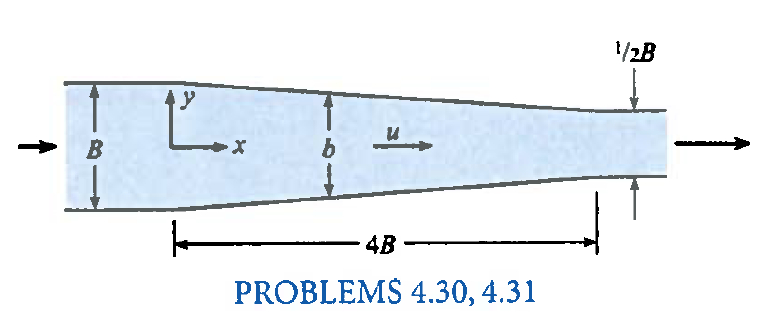
\includegraphics[width=4in]{Nozzle.jpg} 
   \caption{Converging wall flow field}
   \label{fig:Nozzle}
\end{figure}

~
\end{enumerate}


\end{document}  